% description of block structure 

% block diagram
\begin{figure}[ht]
    \centering
    
\begin{tikzpicture}[scale=0.67, every node/.style={transform shape}]
    % macro block diagram for simulation

    \node[block, minimum width=22cm ] (cpp) at ( 2,  0.9) {C++ Wrapper};
    
    % blocks part of the display super-module
    \node[block, minimum width=22cm ] (main) at ( 2, -2.5) {Verilog Wrapper};
    \node[block] (sync) at (-7, -6) {Synchronization module};
    \node[block] (vga) at (-3, -6) {VGA Controller};
    \node[block] (fr) at (-3, -9) {Framer};
    
    % blocks part of the logic super-module
    \node[block, minimum height=5cm] (int) at ( 3, -7.5) {Interface Module};
    \node[block] (tetgen) at ( 7, -6.5) {Tetrimino Generation};
    \node[block] (motcon) at ( 7, -8.5) {Motion Control};
    \node[block, minimum height=5cm] (val) at ( 11, -7.5) {Validation Module};

    \node[draw,inner xsep=4mm,inner ysep=7mm,fit=(vga)(fr)(sync), label={-90:Display Control}] (d) {};
    \node[draw,inner xsep=4mm,inner ysep=7mm,fit=(int)(tetgen)(motcon)(val), label={-90:Game Logic}] (l) {};
    
    \node[draw,inner xsep=4mm,inner ysep=7mm,fit=(main)(d)(l), label={-90:Verilog}] (v) {};

    % super-module connections
    \draw[->] (cpp)-- (main);
    \draw[<->] (vga)-- (vga|- main.south);
    \draw[<->] (int)-- (int|- main.south);

    % display connections
    \draw[<->] (vga.west)-- (sync.east|- vga.west);
    \draw[<->] (fr)-- (vga);

    % logic connections
    \draw[<->] (tetgen)-- (int);
    \draw[<->] (motcon)-- (int);
    \draw[<->] (tetgen)-- (val);
    \draw[<->] (motcon)-- (val);

\end{tikzpicture}

    %\captionsetup{justification=centering}
    \caption{Block diagram $\sankalp{Better\ caption?}$}
\label{fig:blockdiag}
\end{figure}

% verilog
\subsection{Verilog Modules}

% wrapper
\subsubsection{Wrapper}
%
\begin{lstlisting}[language=Verilog]
    input clock;
    input [3:0] actions; // input user action [ROTATE | DOWN | LEFT | RIGHT]
    output vsync;
    output hsync;
    output vga_r;
    output vga_g;
    output vga_b;
    output [7:0] score;
    output gameover;
\end{lstlisting}

Verilog modules are instantiated top-down for the purposes of the 
simulation. The logical structure of the design leaves us with 
several root modules, both harder to manage in practice, and 
unsupported as of yet for the purposes of simulation \cite{verilatortopmod}.
So we create a module that accepts inputs from the C++ wrapper (\ref{subsection:cppwrap}),
provides outputs to it, and acts as an interfacing media for the different
modules, with necessary root modules instantiated within this wrapper.

% logic supermodule
\subsubsection{Logical Modules}
\label{subsection:logicalmod}
\subsubsection{Structural Description}
\label{subsubsection:Structuraldescr}
\begin{lstlisting}[language=Verilog]
    input wire [4:0] operation,  
    input wire vsync, 
    input reg [10:0] framenumber, 
    output reg [2:0] currentstate[0:9][0:19], 
    output reg [7:0] score,
    output reg gameover,
    input clock
\end{lstlisting}
The logical module for the game consists of a single module that takes inputs from the top level wrapper and outputs the board state to the frame buffer. \newline
along with the gamescore and a gameover state. The \code{vsync} acts as the clock that drives the game.

Further, there are several internal components 
\begin{lstlisting}[language=Verilog]
    reg [2:0] tetrimino;
    reg frozen;
    reg [2:0] num_deleted;
    reg [4:0] centerofmass [0:1][0:3]
\end{lstlisting}
These parameters store the coordonites and type of the falling tetrimino and use it for


\subsubsection{Interface}
\label{subsubsection:interface}
The instantiation of the module sets all the registers in the boardstate to 0. An initial tetrimino is generated.
\newline 
When the gameclock updates module performs certain tasks 
\begin{itemize}
    \item Check whether the current tetrimino is frozen or can move more
    \item If it is frozen, check whether the game is over checking whether any block of the top row is filled
    \item If the game isn't over, delete the rows that are filled, update the score ,move all rows above down, generate a new tetrimino
    \item If the tetrimino isn't frozen, move it down 
\end{itemize}
We faced issues issues with the syncing of the actions and input due to the relatively low framerate of the clock. 
Therefore evaluating of the inputs is instead done at negedge vsync to prevent inputs 
from being evaluated simultaneously with the above evaluations.
\subsubsection{Tetrimino Generation }
\label{subsubsection:tetgen}
The inital block is generated as a L-Block. 
Every subsequent block is generated based on the framenumber 
at which the generation happens, which ensures sufficient percieved 
randomness using a simple hashing
 \( \texttt{(Framenumber * PrimeNumber\ \%\ 7) + 1} \) 
With the center of mass at (0,5).
\subsubsection{Motion Control }
\label{subsubsection:motioncontrol}
4 operations are allowed
\begin{itemize}
    \item Move down
    \item Move left
    \item Move Right
    \item Rotate Clockwise
\end{itemize}
 A tempory set of coordinates is created based on the current coordinates of the tetrimino and the operation 
 \begin{itemize}
     \item If the operation is to move left, right or down, all the 4 blocks in the tetrimino are moved by 1 block in the appropriate direction
     \item If the operation is to rotate, the center of mass remains constant while the other 3 blocks rotate clockwise by 90 degrees around the center of mass
 \end{itemize}
 If the operation is found to be valid, the coordinates are updated to
 be equal to the temporary coordinates previously calculated and the boardstate is updated by deleting the blocks at the previous coordinates
 and creating a tetrimino at the new coordinates

\subsubsection{Validation }
\label{subsubsection:validation}
Two things are checked to see whether a move is valid 
\begin{itemize}
    \item Whether the new position goes beyond the boundary. 
    by checking  whether the coordinates are greater than 9 and 19 respectively
    \item Whether the new position overlaps with an occupied block. 
   
\end{itemize}

% display supermodule
\subsubsection{Display Modules}
\label{subsection:display}

\subsubsection{VGA Control Module}
\label{subsubsection:vgacontrol}
%
\begin{lstlisting}[language=Verilog]
    input clock;
    input reg [2:0] frame_buffer [0:9] [0:19], // frame [x][y][R | G | B]
    output reg [2:0] vga_pixel, // output bus for 3-bit RGB color
    output hsync_out;
    output vsync_out;
\end{lstlisting}

The VGA control module serves as a generator for the serial VGA output 
(ports 3-5) and instantiates the framer (\ref{subsubsection:framer}) and
the synchronisation module (\ref{subsubsection:vgasync}).

Every \(\texttt{vga\_clock}\) (see \ref{paragraph:vgasync}), based on the
current \(\texttt{count\_x}\) and \(\texttt{count\_y}\), the relevant pixel from \\
\(\texttt{frame\_buffer}\) is outputted to the VGA bus.\\
 

\subsubsection{Framer Module}
\label{subsubsection:framer}
%
\begin{lstlisting}[language=Verilog]
    input vsync;
    inout reg [2:0] frame_buffer [0:9] [0:19];
    output reg [2:0] frame_out [0:9] [0:19];
\end{lstlisting}

The Framer Module maintains a frame buffer with controlled public access,
gated using a semaphore \cite{semaphore}. This allows other modules and tasks 
to write directly to the frame buffer instead of maintaining copies of the data 
potentially causing overwriting and synchronisation issues.

The module writes this frame buffer onto an output buffer at \(\texttt{vsync}\), 
in turn sent onto VGA rails serially (\ref{subsubsection:vgacontrol})
over the course of the next frame cycle. After flushing this data, the buffer is cleared,
i.e. written over with black, preparing it for the next output cycle.\\

\subsubsection{Synchronisation Module}
\label{subsubsection:vgasync}
%
\begin{lstlisting}[language=Verilog]
    input clock;
    output vga_clock;
    output hsync;              
    output vsync;               
    output in_display;          
    output reg [9:0] count_x;
    output reg [9:0] count_y;
\end{lstlisting}

The Synchronisation Module receives a \(\texttt{clock}\) signal from
the VGA controller (\ref{subsubsection:vgacontrol}) and calculates several
signals critical to the VGA control flow:

\begin{itemize}
    \item \(\texttt{vga\_clock}\) --- a signal generated by dividing the 
            input \(\texttt{clock}\) signal by a known \(\texttt{multiplier}\)
            variable. The multiplier variable can be easily adjusted at runtime
            to allow for adjusting frame times in the event of a performance
            bottleneck or sudden throttle to prevent a drop in frametimes. This
            is akin to a primitive version of modern Adaptive Syncing \cite{varrefresh},
            now popularized as some technologies built into modern GPUs,
            such as AMD Freesync \cite{freesync} and Nvidia G-Sync \cite{gsync}. 
            Modern implementations instead use a specialised controller on the display
            side as well, communicating actively with its counterpart in the GPU,
            as opposed to our host-only solution.
    \item \(\texttt{vsync / hsync}\) --- sync signals standardized as part of the VGA
            standard \cite{vgastandard}. Intended to be passed via a DAC to the monitor.
            In our implementation, \(\texttt{hsync}\) sees little use other than this,
            while \(\texttt{vsync}\), marking, the end of a frame, is at several points 
            (\ref{subsubsection:interface}, \ref{subsubsection:motioncontrol}, \ref{subsubsection:framer}, 
            \ref{subsection:cppwrap}) used to flush a frame buffer or to advance a logical step.
\end{itemize}


% c++
\subsection{C++ Wrapper}
\label{subsection:cppwrap}

In the absence of an FPGA to run described modules, 
we had to look to other options. With a strong desire to 
maintain real-time playability, we tried several options ---
standard simulations had to be rejected due to not being 
anywhere close to real-time, with the inability to accept inputs.
Having considered the idea of running a simulated clock, we then
moved to forcefully driving a clock for the simulation. We attempted
to use \(\texttt{verilog-vga-simulator}\) \cite{vga-simulator},
a C-based program interfacing with the simulation via 
Verilog Procedural Interface (VPI) \cite{vpi}, drawing the resultant
VGA output via Simple DirectMedia Layer \cite{sdl} referred to as 
SDL herein. We were driven away by a cocktail of issues --- primarily
the performance, combined with the relative inflexibility of VPI 
and the now obsolete \cite{sdl_obsolete} SDL API. However, the cocktail
was more than resolvable.

Saving grace came in the form of Verilator \cite{verilator}, a compiler for
Verilog which translates modules top-down into C++ code with
I/O interfaces handled via classes \cite{verilator-implement}. This allowed
us to bypass having to deal with VPI's idiosyncrasies and limited nature, paired
with the finicky fixes required to obtain a realtime driven clock.

Armed with a way to handle inputs and outputs to our modules in realtime, we 
needed a VGA simulator to handle the outputs. This was executed using
SDL2 \cite{sdl2} and a low-level frame-buffer, rendering to screen via 
a cross-platform hardware accelerated rendering interface (with OpenGL \cite{opengl}
primarily used for testing).

\begin{figure}[h]
    \centering
    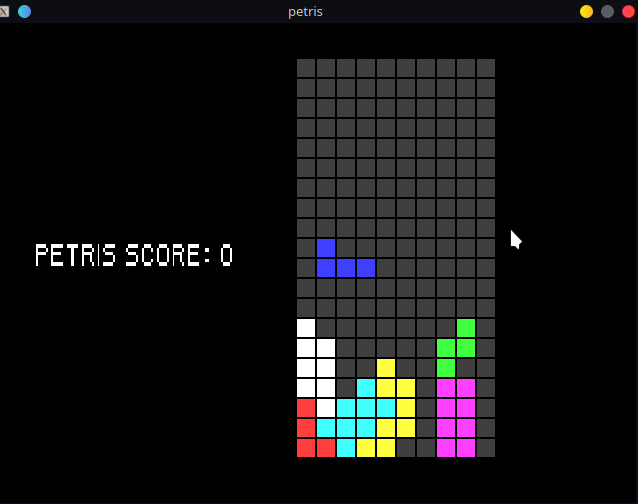
\includegraphics[scale=0.6]{fig/ouput_screenshot.png}
    \caption{SDL based output}
\label{fig:output}
\end{figure}

However, a software based simulation is unable to drive a clock fast enough
to run a VGA simulation in any of the common modes \cite{vga_modes}. As such,
a myriad of performance-centric changes had to be made. Alongside several
minor optimizations was a major change to the system --- a drastic reduction in
resolution or frame rate. Realistically, keeping the same resolution, the frame 
rate would have been cut to approximately \(\texttt{1/20 fps}\), far from playable.
The resolution would have to be cut similarly to maintain a playable frame rate.
Since most of our clock cycles are used up driving the VGA controller, keeping true
to the design, we chose to downscale it. Outputting a much smaller resolution from
the simulated Verilog modules and writing an integer scaling \cite{intscale} system
within the relatively fast C++ wrapper. 

We would like to add that much higher raw resolution and frame rates are possible 
and have been seen after removing the limitation to output serial VGA. Providing
the frame buffer as output to the display simulator in parallel reduces the time
complexity of drawing a frame from \(\bigO (n^2)\) to \(\bigO (1)\) in screen 
dimensions. However, having achieved desired levels of responsiveness and 
playability without resorting to bending the limits of the project, we chose not 
to do this.